%include part: see main.beamer.tex and main.article.tex
%include common packages and settings
\usepackage{etex} %эта магическая херь избавляет от переполнения регистров TeX а!!!

\mode<article>{\usepackage{fullpage}}
\mode<presentation>{
    \usetheme{Madrid} %%Boadilla,Madrid,AnnArbor,CambridgeUS,Malmoe,Singapore,Berlin
    \useoutertheme{shadow}
} 

\usepackage[utf8]{inputenc}
\usepackage[russian]{babel}
\usepackage{indentfirst}
\usepackage{graphicx}

\usepackage{amsmath}
\usepackage{amsfonts}
\usepackage{amsthm}
\usepackage{algorithm}
\usepackage{algorithmic}

\usepackage[all]{xy}

\date{Лекция по дисциплине <<дискретная математика>>\\(\today)}
\author[М.~М.~Шихов]{Михаил Шихов \\ \texttt{\underline{m.m.shihov@gmail.com}}}

%для рисования графов пакетом xy-pic
\entrymodifiers={++[o][F-]}

%для псевдокода алгоритмов (algorithm,algorithmic)
\renewcommand{\algorithmicrequire}{\textbf{Вход:}}
\renewcommand{\algorithmicensure}{\textbf{Выход:}}
\renewcommand{\algorithmiccomment}[1]{// #1}
\floatname{algorithm}{Псевдокод}



\title[Основы алгебры логики]{Основы алгебры логики}

\newcommand{\MyLand}{\cdot}

\begin{document}

%титул и содержание статьи
\mode<article>{\maketitle\tableofcontents}

%титул и содержание презентации
\frame<presentation>{\titlepage}
\begin{frame}<presentation>
    \frametitle{Содержание}
    \tableofcontents
\end{frame}


\section{Логические функции}


\subsection{Основы}

\begin{frame}
    \frametitle{Область определения и область значения}
    
    \begin{itemize}
        \item Любое логическое выражение \alert{истинно} либо \alert{ложно}.
        \item Обозначим истину символом $1$, а ложь --- символом $0$.
    \end{itemize}

    \alert{Логическими функциями} называются функции вида 
    \[
        f(x_1,\ldots,x_n),
    \]
    где, как аргументы $x_i$, так и функция принимают значение либо $0$, либо $1$.
\end{frame} 


\begin{frame}
    \frametitle{Способы задания логических функций}
    \framesubtitle{Таблица истинности}

    \[
        \begin{array}{cccc|c}
            x_1 &\cdots&x_{n-1} &x_n&f(x_1,\cdots,x_{n-1},x_n)\\
            \hline
            0   &\cdots&0       &0  &y_0=f(0,\cdots,0,0)\\
            0   &\cdots&0       &1  &y_1=f(0,\cdots,0,1)\\
            0   &\cdots&1       &0  &y_2=f(0,\cdots,1,0)\\
            0   &\cdots&1       &1  &y_3=f(0,\cdots,1,1)\\
            \cdots   &\cdots&\cdots       &\cdots  &\cdots\\
            1   &\cdots&1       &1  &y_{2^n-1}=f(1,\cdots,1,1)\\
            \hline
        \end{array}
    \]
    
    \uncover<1>{Каково количество всех возможных функций $n$ аргументов?}
    \uncover<2>{
        Количество всех возможных функций $n$ аргументов:
        \[
            2^{2^{n}}.
        \]
    }
\end{frame}


\subsection{Важнейшие логические функции}

\begin{frame}
    \frametitle{Функции одного аргумента}
    
    Функций одного аргумента $f(x)$ всего $2^{2^{1}}=4$. Некоторые не представляют практического интереса, хотя и имеют название:
    \begin{enumerate}
        \item \alert{Константа нуля} для любого аргумента вернёт $0$: $f(x)=0$.
        \item \alert{Константа единицы} для любого аргумента вернет $1$: $f(x)=1$, 
        \item \alert{Тождественная функция} вернет значение аргумента: $f(x)=x$.
    \end{enumerate}
\end{frame}

\begin{frame}
    \frametitle{Функции одного аргумента}
    \framesubtitle{Отрицание, \textit{НЕ}, \textit{NOT}}

    \[
        \begin{array}{ccc}
            \begin{array}{c|c}
                x_1&\textit{не}(x_1)\\
                \hline
                0&1\\
                1&0\\
                \hline
            \end{array}
            &&
            \raisebox{-.7\height}{
                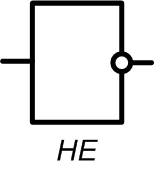
\includegraphics[width=.17\textwidth]{fig/not}
            }
        \end{array}
    \]
    
    <<$\textit{НЕ}(x)$>> также обозначается: <<$\lnot x$>>, <<$\overline{x}$>>.
\end{frame}

\begin{frame}
    \frametitle{Функции двух аргументов}
    
    Из $2^{2^2}=16$ функций двух аргументов лишь $9$ имеют название (см., например, \cite{bib:novic:discrmathprogrammer}).
\end{frame}


\begin{frame}
    \frametitle{Функции двух аргументов}
    \framesubtitle{Конъюнкция, \textit{И}, \textit{AND}}

    \[
        \begin{array}{ccc}
            \begin{array}{cc|c}
                x_1&x_2&\textit{и}(x_1,x_2)\\
                \hline
                0&0&0\\
                0&1&0\\
                1&0&0\\
                1&1&1\\
                \hline
            \end{array}
            &&
            \raisebox{-.7\height}{
                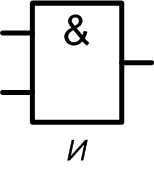
\includegraphics[width=.17\textwidth]{fig/and}
            }
        \end{array}
    \]
    
    <<$\textit{и}(x,y)$>> также обозначается: <<$x\land y$>>, <<$x \& y$>>,  <<$x \MyLand y$>> или  <<$xy$>>.
\end{frame}

\begin{frame}
    \frametitle{Функции двух аргументов}
    \framesubtitle{Дизъюнкция, \textit{ИЛИ}, \textit{OR}}
    
    \[
        \begin{array}{ccc}
            \begin{array}{cc|c}
                x_1&x_2&\textit{или}(x_1,x_2)\\
                \hline
                0&0&0\\
                0&1&1\\
                1&0&1\\
                1&1&1\\
                \hline
            \end{array}
            &&
            \raisebox{-.7\height}{
                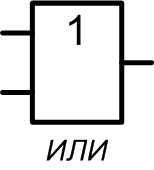
\includegraphics[width=.17\textwidth]{fig/or}
            }
        \end{array}
    \]
    
    <<$\textit{или}(x,y)$>> также обозначается: <<$x \lor y$>>.
\end{frame}

\begin{frame}
    \frametitle{Функции двух аргументов}
    \framesubtitle{<<Исключающее или>>, <<сложение по модулю два>>, \textit{XOR} --- eXclusive OR}
 
    \[
        \begin{array}{ccc}
            \begin{array}{cc|c}
                x_1&x_2&\textit{xor}(x_1,x_2)\\
                \hline
                0&0&0\\
                0&1&1\\
                1&0&1\\
                1&1&0\\
                \hline
            \end{array}
            &&
            \raisebox{-.7\height}{
                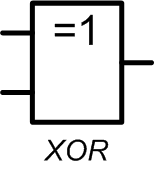
\includegraphics[width=.17\textwidth]{fig/xor}
            }
        \end{array}
    \]
    
    <<$\textit{xor}(x,y)$>> также обозначается: <<$x \oplus y$>>.
    
    Это действительно $\textit{ИЛИ}$, за исключением\footnote{Гораздо проще запомнить эту функцию, как результат сложения в $2$ СС двух бит с отброшенным переносом} того, что $\textit{xor}(1,1)=0$.
\end{frame}

\begin{frame}
    \frametitle{Функции двух аргументов}
    \framesubtitle{Импликация, \textit{ЕСЛИ-ТО}}
    
    \[
        \begin{array}{cc|c}
            x_1&x_2&\textit{если-то}(x_1,x_2)\\
            \hline
            0&0&1\\
            0&1&1\\
            1&0&0\\
            1&1&1\\
            \hline
        \end{array}
    \]
    
    <<$\textit{если-то}(x,y)$>> также обозначается: <<$x \to y$>>.

    Это аналог высказывания <<\alert{если $x_1$, то $x_2$}>>. Оно ложно лишь тогда, когда посылка $x_1$ истинна, а следствие $x_2$ ложно.
\end{frame}

\begin{frame}
    \frametitle{Функции двух аргументов}
    \framesubtitle{Штрих Шеффера, \textit{И-НЕ}}
    
    \[
        \begin{array}{ccc}
            \begin{array}{cc|c}
                x_1&x_2&\textit{и-не}(x_1,x_2)\\
                \hline
                0&0&1\\
                0&1&1\\
                1&0&1\\
                1&1&0\\
                \hline
            \end{array}
            &&
            \raisebox{-.7\height}{
                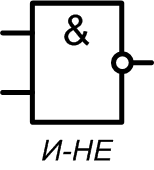
\includegraphics[width=.17\textwidth]{fig/notAnd}
            }
        \end{array}
    \]
    
    <<$\textit{и-не}(x,y)$>> также обозначается: <<$x\mid y$>>.
\end{frame}

\begin{frame}
    \frametitle{Функции двух аргументов}
    \framesubtitle{Стрелка Пирса, \textit{ИЛИ-НЕ}}
    
    \[
        \begin{array}{ccc}
            \begin{array}{cc|c}
                x_1&x_2&\textit{или-не}(x_1,x_2)\\
                \hline
                0&0&1\\
                0&1&0\\
                1&0&0\\
                1&1&0\\
                \hline
            \end{array}
            &&
            \raisebox{-.7\height}{
                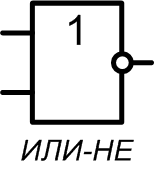
\includegraphics[width=.17\textwidth]{fig/notOr}
            }
        \end{array}
    \]
    
    <<$\textit{или-не}(x,y)$>> также обозначается: <<$x\uparrow y$>>.
\end{frame}


\subsection{Формулы вместо функций трёх и более агрументов}
    
\begin{frame}
    \frametitle{Функции трёх и более аргументов}
    
    Не имеет смысла рассматривать \alert{функции} трех и большего количества аргументов, в силу того, что их можно выразить \alert{формулой}, сконструированной из функций одного и/или двух аргументов.
\end{frame}


\section{Формулы}

\begin{frame}
    \frametitle{Формула}
    
    \alert{Формулой} будем называть выражение 
    \[
        f(t_1,\ldots,t_n),
    \]
    где $t_i$ --- \alert{подформула}, т.е. либо аналогичного вида формула, либо переменная, принимающая одно из значений $0$, либо $1$.

    Прежде чем найти значение формулы, нужно найти значения подформул, стоящих в аргументах.
\end{frame}

\begin{frame}
    \frametitle{Пример формулы}
    
    \begin{example}[Задача] 
        Найти значение формулы 
        \[
            \textit{или}(0,\textit{и}(\textit{не}(1), 1)).
        \]
    \end{example}
    \begin{proof}<2>[Решение] 
        \(
            \textit{или}(0,\textit{и}(\textit{не}(1), 1))\Rightarrow
            \textit{или}(0,\textit{и}(0, 1))\Rightarrow
            \textit{или}(0,0)\Rightarrow 0
        \)
    \end{proof}
\end{frame}


\subsection{Конструирование функций формулами}

\begin{frame}
    \frametitle{Конструирование функций формулами}
    
    Функции произвольного количества аргументов можно конструировать на основе вышеназванных функций одного и двух аргументов. 
    \begin{example} 
        Функция трёх аргументов задана формулой:
        \[
            g(x_1,x_2,x_3)=\textit{или}(x_1,\textit{и}(\textit{не}(x_2), x_3)).
        \]
    \end{example}
\end{frame}


\subsection{Запись формул}

\begin{frame}
    \frametitle{Символы операций вместо функций}
    
    Вместо
    \begin{enumerate}
        \item{} <<$\textit{не}(x)$>> пишут <<$(\lnot x)$>> или <<$(\bar{x})$>>;
        \item{} <<$\textit{и}(x,y)$>> пишут <<$(x \land y)$>>, <<$(x \& y)$>>,  <<$(x \MyLand y)$>> или  <<$(xy)$>>;
        \item{} <<$\textit{и-не}(x,y)$>> пишут <<$(x \mid y)$>>;
        \item{} <<$\textit{или}(x,y)$>> пишут <<$(x \lor y)$>>;
        \item{} <<$\textit{или-не}(x,y)$>> пишут <<$(x \uparrow y)$>>.
        \item{} <<$\textit{xor}(x,y)$>> пишут <<$(x \oplus y)$>>;
        \item{} <<$\textit{если-то}(x,y)$>> пишут <<$(x \to y)$>>;
    \end{enumerate}

    Задавая приоритет операций, лишние скобки опускают.
    \begin{example} 
        {}<<$\lnot x\lor y\MyLand z$>> то же самое, что <<$(\lnot x)\lor (y\MyLand z)$>>.
    \end{example}
\end{frame}

\begin{frame}
    \frametitle{Операции вместо функций}
    
    \begin{example}
        Функция 
        \[
            g(x_1,x_2,x_3)=\textit{или}(x_1,\textit{и}(\textit{не}(x_2), x_3))
        \]
        может быть записана с помощью обозначений операций:
        \[
            g(x_1,x_2,x_3) = \only<1>{?}\only<2->{x_1 \lor \lnot x_2 \MyLand x_3}
        \]
    \end{example}
    
    \begin{center}
        \uncover<2>{ Какая логическая схема реализует $g(x_1,x_2,x_3)$? }
        \uncover<3>{ 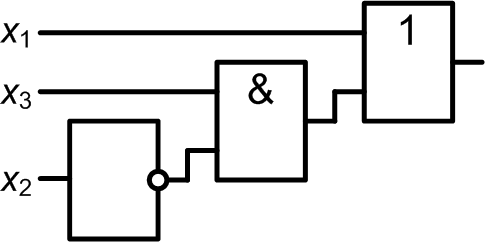
\includegraphics[width=.42\textwidth]{fig/formulae} }
    \end{center}
\end{frame}

\begin{frame}
    \frametitle{Ассоциативные операции}
    \framesubtitle{Элементы цифровой техники}

    Такие операции как \textit{И}, \textit{ИЛИ}, \textit{XOR} ассоциативны. То есть, например,
    \[
        (x\MyLand y)\MyLand z = x\MyLand (y\MyLand z) = x\MyLand y\MyLand z.
    \]
    
    Поэтому на схемах допустимы трех и более-входовые элементы\footnote{Которым соответствуют микросхемы, шаблоны ПЛИС и т.д.}:
    \begin{center}
        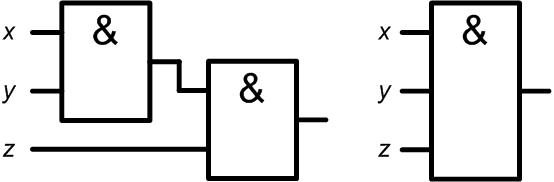
\includegraphics[width=.6\textwidth]{fig/tripleAnd}
    \end{center}
\end{frame}

\subsection{Алгебра логики}

\begin{frame}[allowframebreaks]
    \frametitle{Алгебра логики}
    \framesubtitle{Свойства операций}
    
    \begin{enumerate}
        \item Ассоциативность:
            \[x_1\MyLand(x_2\MyLand x_3) = (x_1\MyLand x_2)\MyLand x_3;\quad x_1\lor(x_2\lor x_3) = (x_1\lor x_2)\lor x_3.\] 
            
        \item Коммутативность:
            \[x_1\MyLand x_2 = x_2\MyLand x_1;\quad x_1\lor x_2 = x_2\lor x_1.\] 
         
        \item Дистрибутивность:
            \[  x_1\MyLand (x_2\lor x_3) = (x_1\MyLand x_2)\lor(x_1\MyLand x_3);
                \quad x_1\lor (x_2\MyLand x_3) = (x_1\lor x_2)\MyLand(x_1\lor x_3).\] 
         
        \item Идемпотентность:
            \[x\MyLand x = x;\quad x\lor x = x.\] 
            
        \item Двойное отрицание:
            \[\overline{\overline{x}} = x.\] 
            
        \item Свойства констант:
            \begin{align*}
                &x\MyLand 1 = x; & &x\MyLand 0 = 0;      & & x\lor 1 = 1 \\
                &x\lor 0 = x;  & &\overline{0} = 1;  & & \overline{1} = 0
            \end{align*}
            
        \item Закон де Моргана:
            \[\overline{x_1\MyLand x_2} = \overline{x_1}\lor \overline{x_2};\quad \overline{x_1\lor x_2} = \overline{x_1}\MyLand \overline{x_2}.\] 
            
        \item Закон противоречия:
            \[x\MyLand \overline{x} = 0.\] 
            
        \item Закон <<исключённого третьего>>:
            \[x\lor \overline{x} = 1.\] 
    \end{enumerate}
\end{frame}

\begin{frame}[allowframebreaks]
    \frametitle{Алгебра логики}
    \framesubtitle{Упрощение формул}
    
    \begin{enumerate}
        \item Поглощение:
            \[x\lor(x\MyLand y) = x; \quad x\MyLand(x\lor y) = x.\] 
            
        \item Склеивание:
            \[(x\MyLand y)\lor(x\MyLand\overline{y}) = x.\] 
            
        \item Обобщённое склеивание:
            \begin{align*}
                &(x\MyLand z)\lor(y\MyLand\overline{z})\lor(x\MyLand y) = (x\MyLand z)\lor(y\MyLand \overline{z});\\
                &x\lor(\overline{x}\MyLand y)=x\lor y;\\
                &x_1\lor f(x_1,x_2,\ldots,x_n) = x_1\lor (\overline{x_1}\MyLand f(0,x_2,\ldots,x_n))\lor\\
                &\lor (x_1\MyLand f(1,x_2,\ldots,x_n)) = x_1\lor f(0,x_2,\ldots,x_n).
            \end{align*}
    \end{enumerate}
\end{frame}

\section{Базис}

\subsection{Основной логический базис}

\begin{frame}
    \frametitle{Основной логический базис}
    
    Функции \textit{И}, \textit{ИЛИ}, \textit{НЕ} составляют \alert{основной логический базис}. Любую функцию можно выразить формулой на их основе. Эти логические связки часто используются в обыденной жизни.
\end{frame}

\begin{frame}
    \frametitle{Основной логический базис}
    \framesubtitle{Конструирование функций трёх и более аргументов}
    
    \begin{example}[Задача] 
        Представить функцию $f(x_1,x_2,x_3)$ в основном логическом базисе.
        \[
            \begin{array}{ccc|c}
                x_1&x_2&x_3&f(x_1,x_2,x_3)\\
                \hline
                0&0&0&0\\
                0&0&1&0\\
                0&1&0&1\\
                0&1&1&0\\
                1&0&0&0\\
                1&0&1&0\\
                1&1&0&1\\
                1&1&1&0\\
                \hline
            \end{array}    
        \]
    \end{example}
\end{frame}

\begin{frame}
    \frametitle{Основной логический базис}
    \framesubtitle{Конструирование функций трёх и более аргументов}
    
    \begin{proof}[Решение]
        На наборе $x_1=0$, $x_2=1$, $x_3=0$ функция $f(x_1,x_2,x_3)$ должна равняться единице. При этом видно, что функция $f_2(x_1,x_2,x_3)=\overline{x_1}\MyLand x_2 \MyLand\overline{x_3}$ равняется единице только на этом наборе. $f(x_1,x_2,x_3)$ также должна равняться $1$ на наборе $x_1=1$, $x_2=1$, $x_3=0$. $f_6(x_1,x_2,x_3)=x_1\MyLand x_2 \MyLand\overline{x_3}$. Стало быть\footnote{Конечно, это решение можно оптимизировать. Вдумавшись, можно видеть, что от $x_1$ функция не зависит: $f(x_1,x_2,x_3)=x_2 \MyLand\overline{x_3}$. Такое представление называется ДНФ --- дизъюнктивная нормальная форма. Оптимизацию формул здесь не рассматриваем} $f(x_1,x_2,x_3)=f_2(x_1,x_2,x_3)\lor f_6(x_1,x_2,x_3)=(\overline{x_1}\MyLand x_2 \MyLand\overline{x_3})\lor(x_1\MyLand x_2 \MyLand\overline{x_3})$.
    \end{proof}
\end{frame}

\subsection{Избыточность основного логического базиса}

\begin{frame}
    \frametitle{Основной логический базис}
    \framesubtitle{Избыточность основного логического базиса}
    
    Например, функцию \textit{И} можно выразить через функции \textit{ИЛИ} и \textit{НЕ}:
    \[x_1\MyLand x_2 = \overline{\overline{x_1}\lor\overline{x_1}},\] 
    в чём нетрудно убедиться непосредственной проверкой:
    \[
        \begin{array}{c|cc|c}
            x_1\MyLand x_2&x_1&x_2&\overline{\overline{x_1}\lor\overline{x_1}}\\
            \hline
            0&0&0&0\\
            0&0&1&0\\
            0&1&0&0\\
            1&1&1&1\\
            \hline
        \end{array}
    \]
    
    Следовательно, базис образуют функции \textit{ИЛИ} и \textit{НЕ}!
\end{frame}

\begin{frame}
    \frametitle{Базис из одной функции}
    \framesubtitle{Стрелка Пирса, \textit{ИЛИ-НЕ}}

    \[
        \begin{array}{cc|c}
            x_1&x_2&x_1\uparrow x_2\\
            \hline
            0&0&1\\
            0&1&0\\
            1&0&0\\
            1&1&0\\
            \hline
        \end{array}
    \]
    
    Достаточно выразить, например функции \textit{НЕ} и \textit{ИЛИ}:
    \begin{itemize}
        \item \textit{НЕ}: $\lnot x=x\uparrow x$;
        \item \textit{ИЛИ}: $x\lor y=\lnot(x\uparrow y)=(x\uparrow y)\uparrow(x\uparrow y)$;
    \end{itemize}

    \begin{center}
        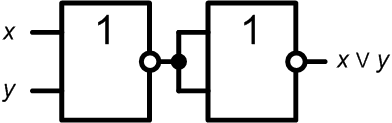
\includegraphics[width=.45\textwidth]{fig/orByNotOr}
    \end{center}
\end{frame}


\appendix

\begin{frame}[fragile]
    \frametitle{Программирование}
    \framesubtitle{Логические операции в ЯВУ и в процессорах}
    
    \begin{center}
        \begin{tabular}{c|l}
            \hline\hline
            Оператор языка C/C++ & Действие оператора\\
            \hline\hline
            \verb"x=y"  &Присвоить переменной \verb"x" значение \verb"y"\\
            \verb"x==y" &Сравнить значения переменных \verb"x" и \verb"y"\\
            \verb"~x"   &Битовое \emph{НЕ}\\
            \verb"x|y"  &Битовое \emph{ИЛИ}\\
            \verb"x&y"  &Битовое \emph{И}\\
            \verb"x^y"  &Битовое \emph{XOR}\\
            \verb"x<<n" &Сдвиг значения \verb"x" на \verb"n" бит влево\\
            \verb"x>>n" &Сдвиг значения \verb"x" на \verb"n" бит вправо\\
            \hline
        \end{tabular}
    \end{center}    
\end{frame}

\begin{frame}[fragile]
    \frametitle{Программирование}
    \framesubtitle{Логические операции в ЯВУ и в процессорах}
    
    \begin{center}
        \begin{tabular}{lcccccccccc}
                     &&\small{7}&\small{6}&\small{5}&\small{4}&\small{3}&\small{2}&\small{1}&\small{0}& \\ \cline{3-10}
            \verb"x"    &\multicolumn{1}{c|}{}  &0&0&1&1&1&1&0&0&\multicolumn{1}{|c}{}\\ \cline{3-10}
            \verb"y"    &\multicolumn{1}{c|}{}  &0&1&0&1&1&0&1&0&\multicolumn{1}{|c}{}\\ \cline{3-10}
            \\ \cline{3-10}
            \verb"z1 = ~x"   &\multicolumn{1}{c|}{}  &1&1&0&0&0&0&1&1&\multicolumn{1}{|c}{}\\ \cline{3-10}
            \verb"z2 = x|y"  &\multicolumn{1}{c|}{}  &0&1&1&1&1&1&1&0&\multicolumn{1}{|c}{}\\ \cline{3-10}
            \verb"z3 = x&y"  &\multicolumn{1}{c|}{}  &0&0&0&1&1&0&0&0&\multicolumn{1}{|c}{}\\ \cline{3-10}
            \verb"z4 = x^y"  &\multicolumn{1}{c|}{}  &0&1&1&0&0&1&1&0&\multicolumn{1}{|c}{}\\ \cline{3-10}
            \verb"z5 = x<<1" &\multicolumn{1}{c|}{}  &0&1&1&1&1&0&0&0&\multicolumn{1}{|c}{}\\ \cline{3-10}
            \verb"z6 = x>>2" &\multicolumn{1}{c|}{}  &0&0&0&0&1&1&1&1&\multicolumn{1}{|c}{}\\ \cline{3-10}
        \end{tabular}
    \end{center}
\end{frame}

\begin{frame}
    \frametitle{В заключение}
    
    Основы алгебры логики даны практически во всех учебниках.
    
    Фундаментальное изложение можно найти в \cite{bib:gorbatovs:discrmath, bib:yablonsky:discreteintro}.
    
    С точки зрения программиста в \cite{bib:novic:discrmathprogrammer, bib:haggard:discrmathprogrammer}.
    
    Доступно и кратко в \cite{bib:sudoplatov:discrmath}.
    
    Работа над битами с помощью арифметико-логических команд процессора \cite{bib:warren:algTriks}.
\end{frame}


\begin{frame}[allowframebreaks]{Библиография}
    \bibliographystyle{gost780u}
    \bibliography{./../../bibliobase}
\end{frame}

\end{document}